\section{Visualization}

To compare the observed signal with background noise, both traces were plotted on the same graph. Trace 1 is the data that came
from when the radio telescope was pointed at the target, Trace 2 data came from when the radio telescope was pointed
away from the target.

Plotting both traces in the same graph allows for direct comparison and helps identify potential hydrogen emission.

There are three separate data collections that were analyzed. Two sets came from Cassiopeia A on different days, and one set 
came from Virgo A.

\vspace{0.5cm}

Figure~\ref{fig: CasA1_Data} shows the frequency spectrum for the first Casseiopeia observation.

\begin{figure}[H]
\begin{center}
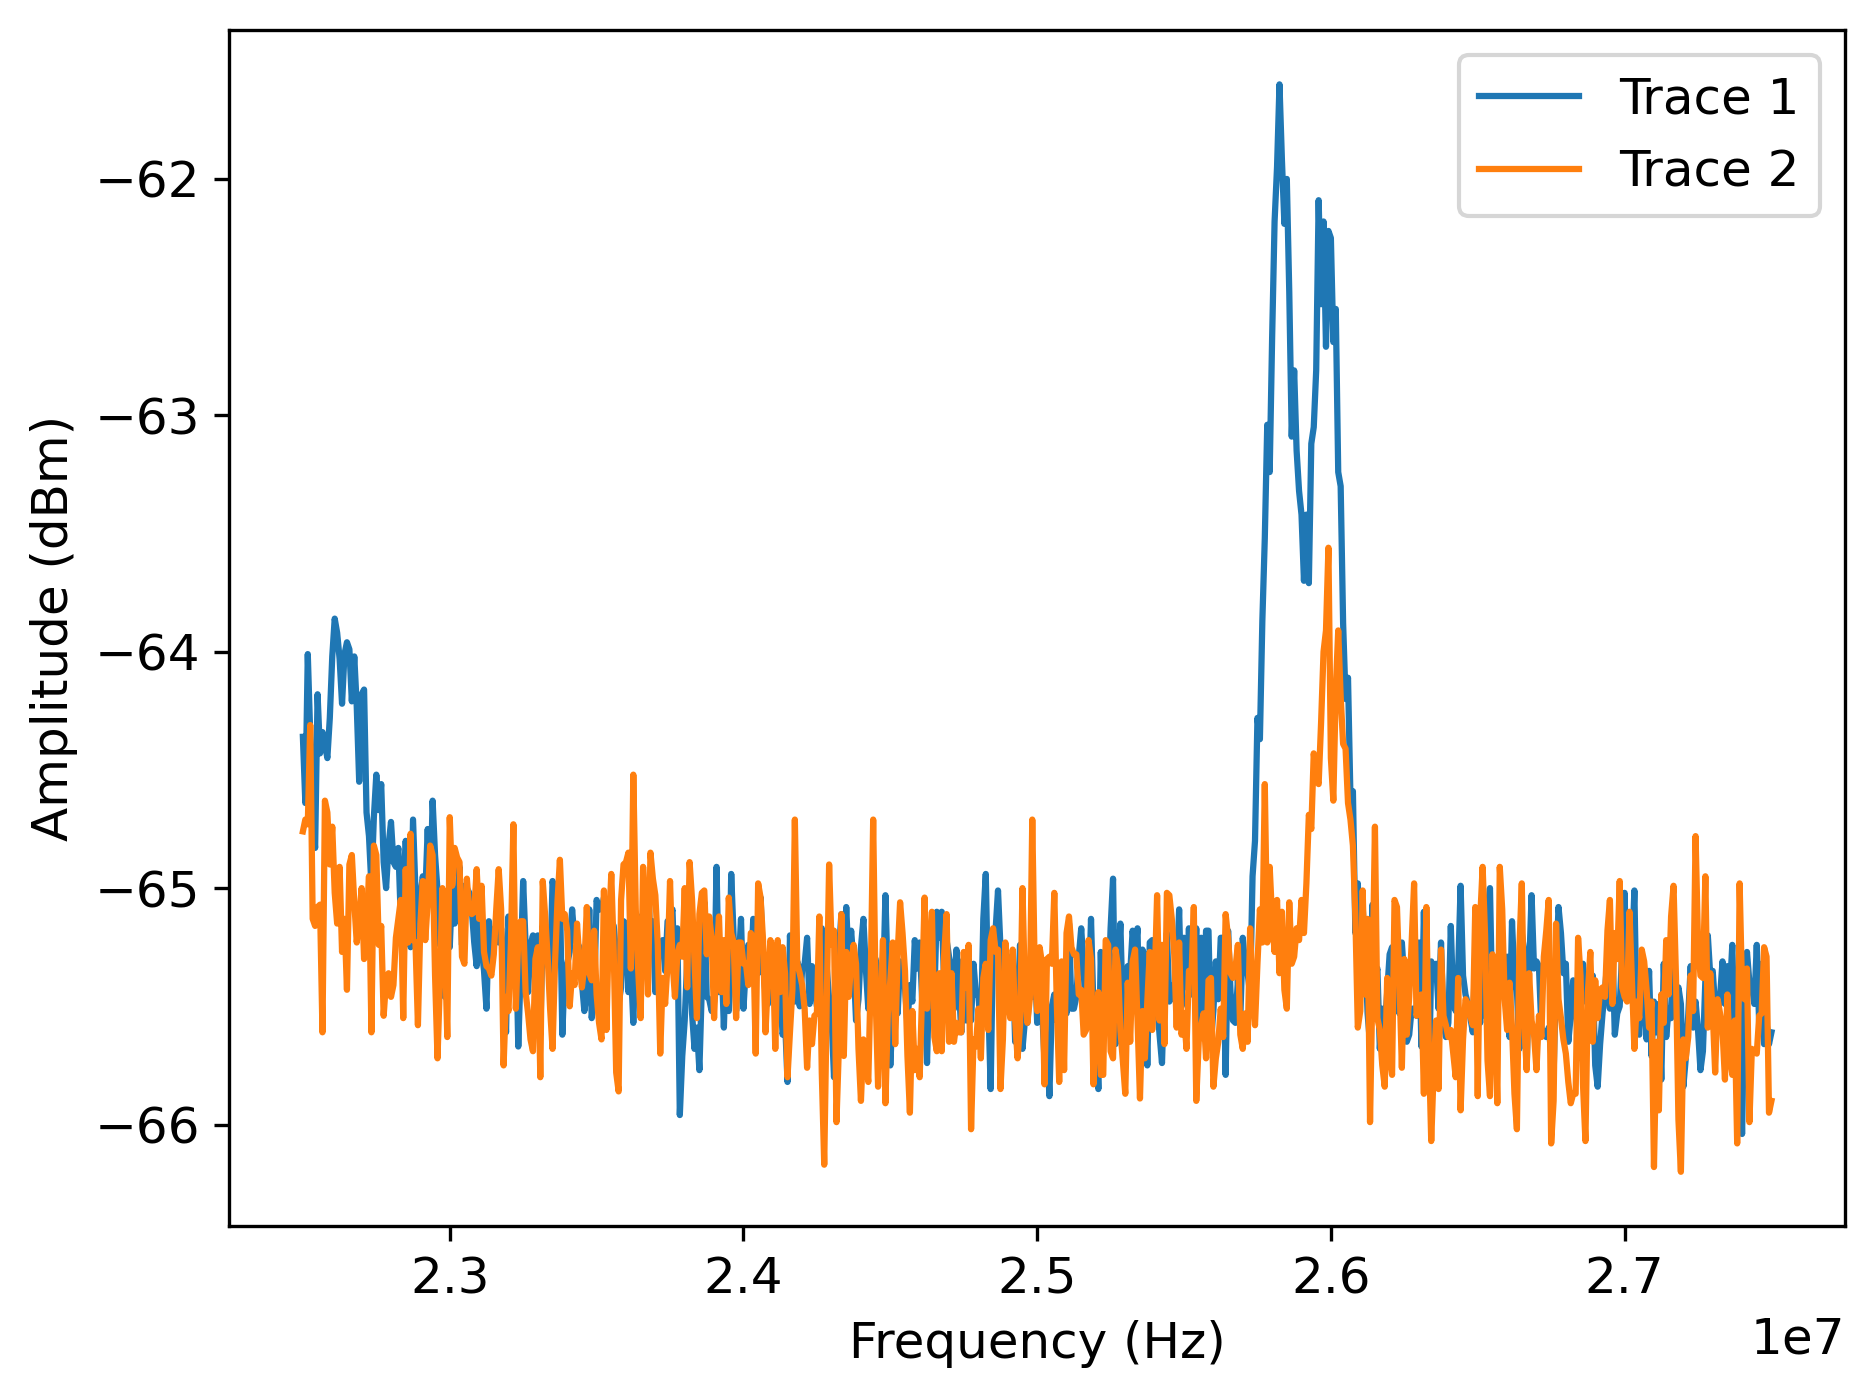
\includegraphics[width=0.85\textwidth]{CasA1_Data.png}
\end{center}
\caption{CasA1 Data}
\label{fig: CasA1_Data}
\end{figure}


Figure~\ref{fig: CasA_040726_Data} shows the frequency spectrum for the casseiopeia observation taken on April 7, 2026. This is the data that shows a potential hydrogen emmission.

\begin{figure}[H]
\begin{center}
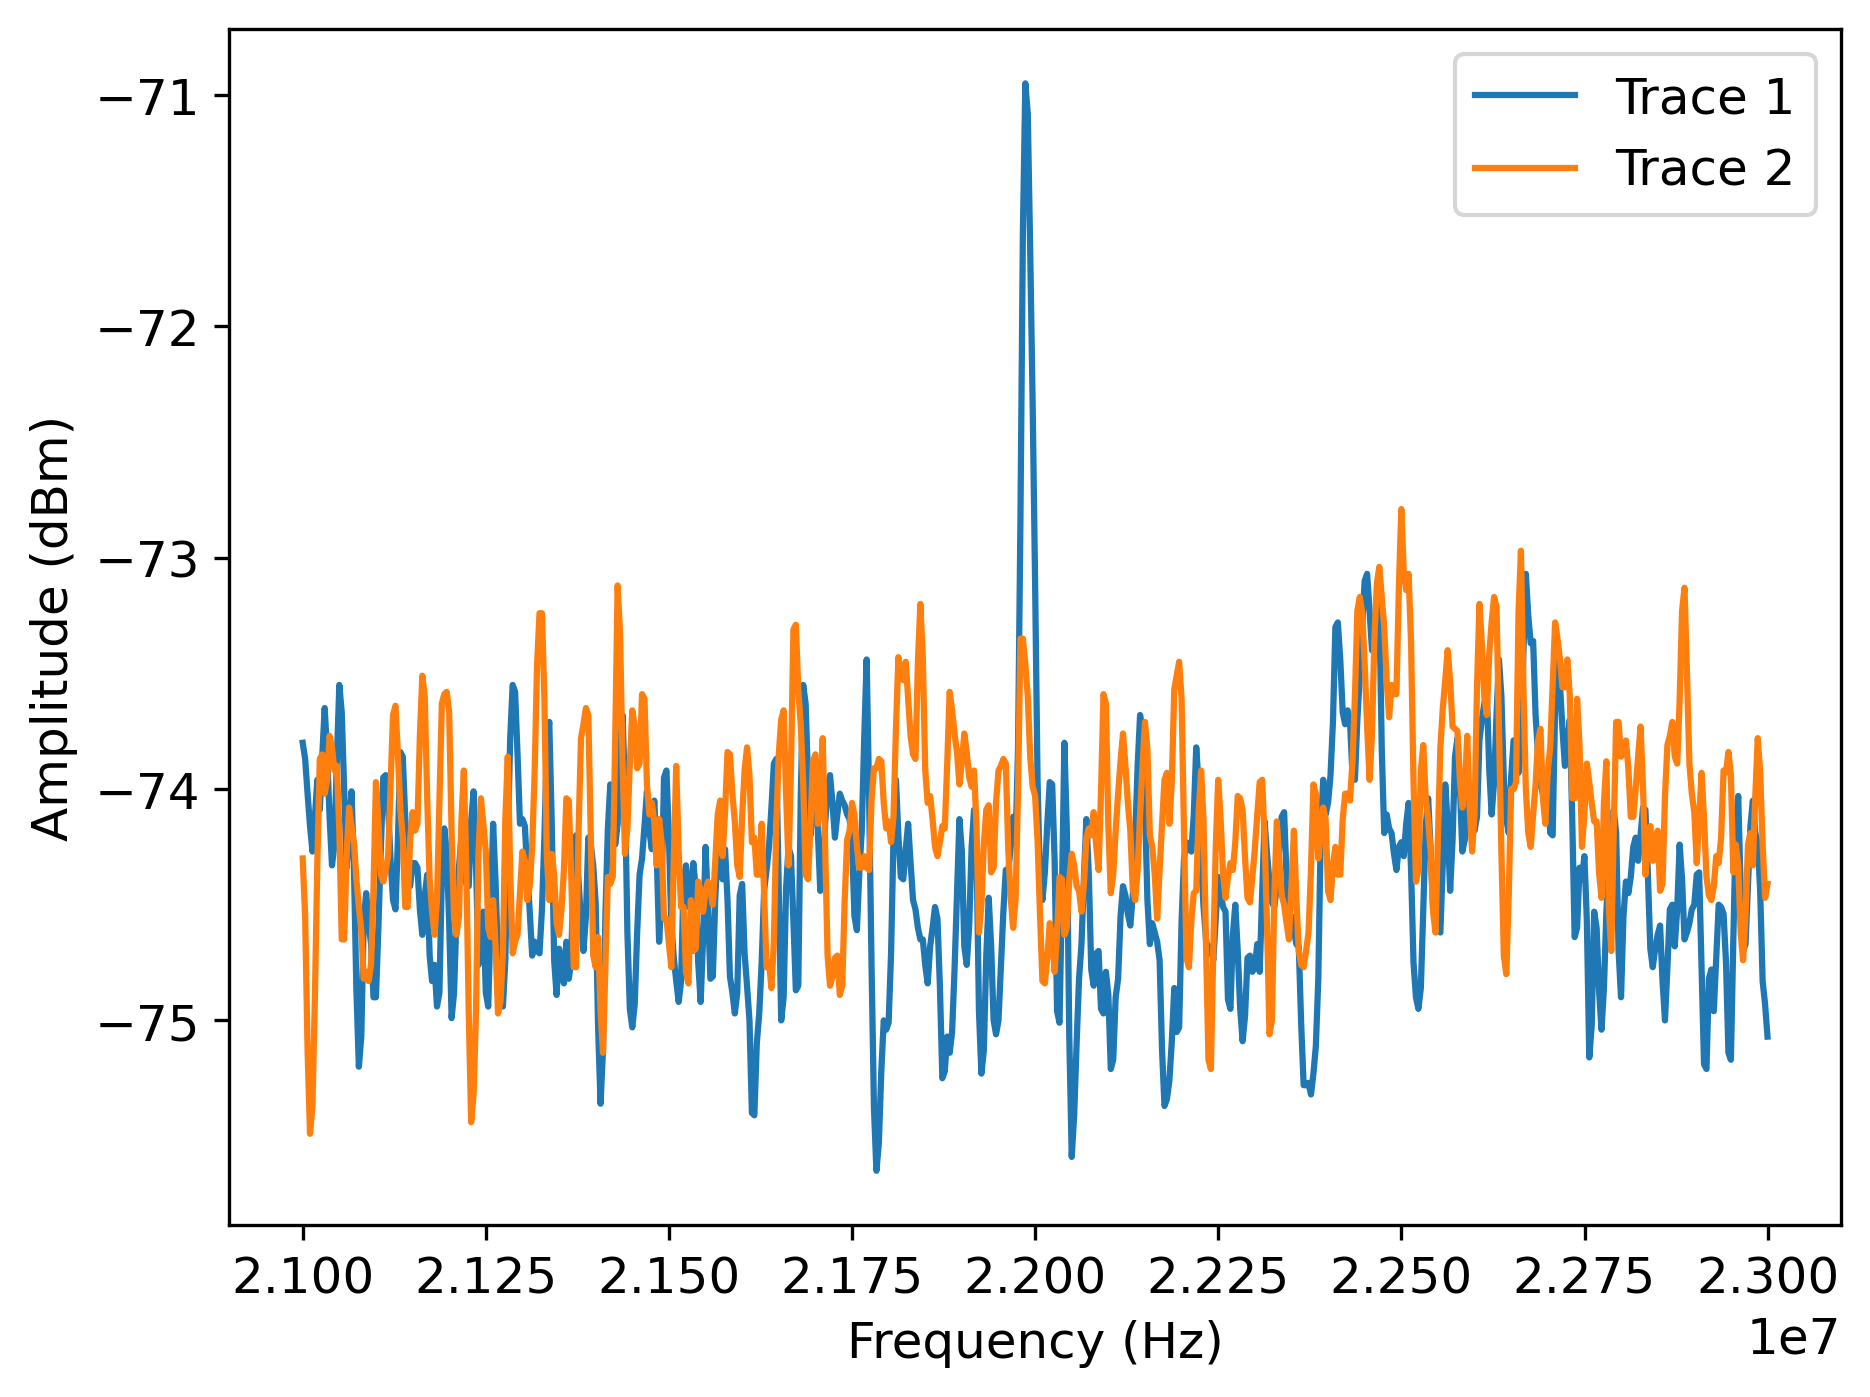
\includegraphics[width=0.85\textwidth]{CasA_040726_Data.png}
\end{center}
\caption{CasA Data from 04/07/26}
\label{fig: CasA_040726_Data}
\end{figure}


Figure~\ref{fig: VirgoA Data} shows the frequency spectrum for the Virgo A observation.

\begin{figure}[H]
\begin{center}
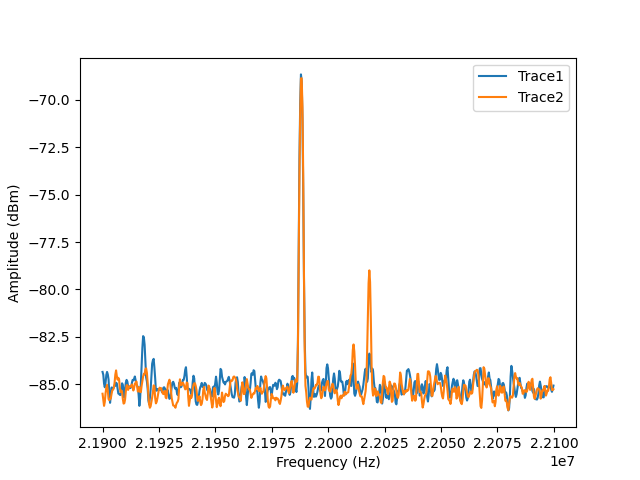
\includegraphics[width=0.85\textwidth]{VirgoA_040726_Data.png}
\end{center}
\caption{VirgoA Data from 04/07/26}
\label{fig: VirgoA Data}
\end{figure}


\clearpage
